\chapter{THUẬT TOÁN DIJKSTRA}

\minitoc

\section{Nguồn tài nguyên}

Nội dung bài chủ yếu tham khảo/copy từ [VNOI WIKI] : \url{https://wiki.vnoi.info/algo/graph-theory/shortest-path}

\section{Thuật toán Dijkstra}


Thuật toán Dijkstra dùng để giải quyết bài toán \textbf{đường đi ngắn nhất một nguồn} (Single-source shortest path) trên đồ thị có \textbf{trọng số không âm}.

\subsection{Bài toán}

Cho một đồ thị có hướng với $N$ đỉnh (được đánh số từ $0$ đến $N-1$), $M$ cạnh có hướng, có trọng số, và một đỉnh nguồn $S$. \textbf{Trọng số của tất cả các cạnh đều không âm.} Yêu cầu tìm ra đường đi ngắn nhất từ đỉnh $S$ tới tất cả các đỉnh còn lại (hoặc cho biết nếu không có đường đi).

\paragraph{Input}
\begin{lstlisting}
7 8 0
0 2 7
0 1 1
0 3 4
2 5 8
5 3 3
4 5 6
1 4 3
2 4 3
\end{lstlisting}
\paragraph{Output}
\begin{lstlisting}
0
1
7
4
4
10
-1
\end{lstlisting}

\begin{figure}[h]
    \centering
    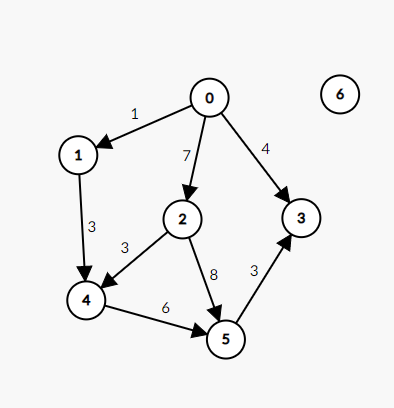
\includegraphics[width=0.4\textwidth]{resource/img/b7/dijkstra_1.png}
    \caption{Minh họa ví dụ}
\end{figure}

 Ở đồ thị này, đỉnh nguồn là đỉnh $0$, đường đi ngắn nhất từ $0$ đến các đỉnh $0$ đến $5$ là $[0, 1, 7, 4, 4, 10]$. Riêng đỉnh $6$ không có đường đi đến.

\subsection{Ý tưởng của thuật toán}

Ý tưởng chính của thuật toán Dijkstra là tối ưu hóa đường đi bằng cách xét các cạnh $(u, v)$, so sánh hai đường đi $S \to v$ sẵn có với đường đi $S \to u \to v$.

Thuật toán sẽ duy trì một mảng chứa đường đi ngắn nhất từ $S$ đến tất cả các đỉnh. Ở mỗi bước, chọn đỉnh $u$ với đường đi $S \to u$ có trọng số nhỏ nhất trong số các đỉnh chưa được xử lý. Sau đó, thuật toán kiểm tra và cập nhật đường đi $S \to v$ bằng cách thử đường đi $S \to u \to v$. Nếu $S \to v$ là đường đi ngắn nhất được tìm ra nhờ không cần kiểm tra lại và được đánh dấu là đã xử lý xong. Thuật toán tiếp tục lặp các bước trên với các đỉnh còn lại cho đến khi tất cả đỉnh đều được xử lý xong.

\subsection{Minh họa thuật toán}

Ta sẽ minh họa thuật toán bằng một đồ thị như hình. Định nghĩa:
\begin{itemize}
    \item $D_u$ là đường đi ngắn nhất từ đỉnh nguồn đến đỉnh $u$ đã tìm được.
    \item $P_u$ nhận hai giá trị $true, false$ cho biết đỉnh $P_u$ đã được chọn để tối ưu chưa.
\end{itemize}

\textbf{Đỉnh được tô đen (đỉnh 0) sẽ là đỉnh nguồn.}

\begin{figure}[h]
    \centering
    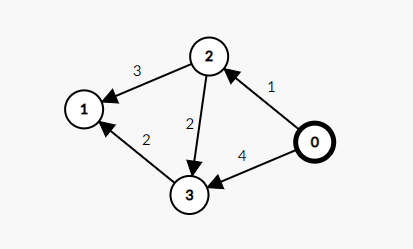
\includegraphics[width=0.4\textwidth]{resource/img/b7/dijkstra_2.png}
\end{figure}
Ban đầu, $D = [0, \infty, \infty, \infty],\; P = [false, false, false, false]$

\begin{itemize}
    \item \textbf{Bước 1:} Thuật toán sẽ chọn đỉnh $0$, vì $D_0 = 0$ là nhỏ nhất thỏa mãn $P_0 = false$. Tiến hành tối ưu các cạnh đi ra:
    \begin{itemize}
        \item Cạnh $(0,2)$: cập nhật $D_2 = \min(D_2, D_0 + W_{0,2}) = \min(\infty, 0+1) = 1$
        \item Cạnh $(0,3)$: cập nhật $D_3 = \min(D_3, D_0 + W_{0,3}) = \min(\infty, 0+4) = 4$
    \end{itemize}
\end{itemize}

Sau bước này, $D = [0, \infty, 1, 4],\; P = [true, false, false, false]$

\begin{itemize}
    \item \textbf{Bước 2:} thuật toán sẽ chọn ra đỉnh $2$, có $D_2 = 1$ là nhỏ nhất thỏa mãn $P_2 = false$. Tiến hành tối ưu các cạnh đi ra:
    \begin{itemize}
        \item Cạnh $(2,1)$: cập nhật $D_1 = \min(D_1, D_2 + W_{2,1}) = \min(\infty, 1 + 3) = 4$
        \item Cạnh $(2,3)$: cập nhật $D_3 = \min(D_3, D_2 + W_{2,3}) = \min(4, 1 + 2) = 3$
    \end{itemize}
\end{itemize}

Sau bước này, $D = [0, 4, 1, 3],\; P = [true, false, true, false]$

\begin{itemize}
    \item \textbf{Bước 3:} thuật toán sẽ chọn ra đỉnh $3$, có $D_3 = 3$ là nhỏ nhất thỏa mãn $P_3 = false$. Tiến hành tối ưu các cạnh đi ra:
    \begin{itemize}
        \item Cạnh $(3,1)$: cập nhật $D_1 = \min(D_1, D_3 + W_{3,1}) = \min(4, 3 + 2) = 4$
    \end{itemize}
\end{itemize}

Sau bước này, $D = [0, 4, 1, 3],\; P = [true, false, true, true]$

\begin{itemize}
    \item \textbf{Bước 4:} thuật toán sẽ chọn đỉnh $1$. Không có cạnh nào đi ra.
\end{itemize}

Đến đây, tất cả các đỉnh đều đã được đánh dấu. Thuật toán kết thúc. Đường đi ngắn nhất tìm được từ đỉnh $0$ là $D = [0, 4, 1, 3]$.

\subsection{Cài đặt}

Ở thuật toán này, ta sẽ lưu đồ thị dưới dạng \textbf{danh sách kề}, trong đó mỗi đỉnh $u$ có danh sách các cặp $(v, w)$ biểu diễn cạnh từ $u$ đến $v$ với trọng số $w$.

Ta định nghĩa các biến như sau:
\begin{itemize}
    \item \textbf{\texttt{dist[u]}} là độ dài đường đi ngắn nhất từ $s \to u$. Ban đầu, ta gán \texttt{dist[u] = oo} với mọi $u$, riêng \texttt{dist[s] = 0}.
    \item \textbf{\texttt{adj[u]}} là danh sách các cặp $(v, w)$ kề với $u$, biểu diễn cạnh có trọng số $w$ nối từ $u \to v$.
    \item \textbf{\texttt{visited[u]}} là mảng đánh dấu các đỉnh đã được xử lý. Ban đầu tất cả đều là \texttt{false}.
    \item \textbf{\texttt{trace[u]}} (nếu cần) lưu đỉnh liền trước $u$ trên đường đi ngắn nhất từ $s$ đến $u$.
\end{itemize}

Thuật toán thực hiện tối đa $n$ bước, mỗi bước gồm:
\begin{itemize}
    \item Tìm đỉnh $u$ sao cho \texttt{visited[u] = false} và \texttt{dist[u]} là nhỏ nhất trong số các đỉnh chưa xử lý.
    \item Duyệt qua các đỉnh $v$ kề với $u$, nếu \texttt{dist[v] > dist[u] + w} thì cập nhật: \\
    \texttt{dist[v] = dist[u] + w} và \texttt{trace[v] = u}.
    \item Đánh dấu \texttt{visited[u] = true}, nghĩa là đỉnh $u$ đã được xử lý xong.
\end{itemize}

\subsection{Độ phức tạp thuật toán}

Trong quá trình tính toán, ta thực hiện $N$ lần lặp:
\begin{itemize}
    \item Bước đầu tiên có độ phức tạp $O(N)$ mỗi lần lặp.
    \item Bước hai hết có tổng độ phức tạp $O(M)$ qua tất cả các lần lặp.
\end{itemize}

Như vậy độ phức tạp của cách cài đặt cơ bản sẽ là $O(N^2 + M)$.

\begin{lstlisting}
#include <bits/stdc++.h>
#define int long long
#define endl "\n"
using namespace std;

const int oo = 1e18;
const int MAXN = 100005;

int n, m, S;
vector< pair<int, int> > adj[MAXN];
vector<int> dist(MAXN, oo), trace(MAXN, -1);
vector<bool> visited(MAXN, false);

void dijkstra(int s) {
    dist[s] = 0;
    for (int i = 1; i <= n; i++) {
        int uBest;
        int Min = oo;
        for (int u = 1; u <= n; u++) {
            if (visited[u] == false && dist[u] < Min) {
                Min = dist[u];
                uBest = u;
            }
        }

        int u = uBest;
        visited[u] = true;

        for (auto x : adj[u]) {
            int v = x.first;
            int w = x.second;
            if (dist[v] > dist[u] + w) {
                dist[v] = dist[u] + w;
                trace[v] = u;
            }
        }
    }
}

signed main() {
    cin >> n >> m >> S;
    for (int i = 1; i <= m; i++) {
        int u, v, w; cin >> u >> v >> w;
        adj[u].push_back({v, w});
    }

    dijkstra(S);

    for (int i = 1; i <= n; i++) {
        if (dist[i] == oo) cout << -1 << " ";
        else cout << dist[i] << " ";
    }
    cout << endl;
}
\end{lstlisting}

\section{Cải tiến đối với đồ thị thưa}

\begin{itemize}
    \item Nhận xét rằng bước đầu tiên: "Tìm đỉnh $u$ có $D_u$ nhỏ nhất và $P_u = false$", có thể được cải tiến. Ta có thể sử dụng cấu trúc dữ liệu \textbf{Heap} (cụ thể là Min Heap) hoặc cây nhị phân tìm kiếm để cải tiến bước này.
    \item Mỗi lần chọn cạnh $(u, v)$ để tối ưu hóa $D_v$, ta đẩy cặp $\{D_v, v\}$ vào trong Heap. Sử dụng $M$ cạnh sẽ có tổng độ phức tạp là $O(M \log N)$.
    \item Để tìm đỉnh có $D_u$ nhỏ nhất, ta chỉ cần liên tục lấy phần tử trên cùng trong Heap ra, cho đến khi gặp đỉnh $u$ thỏa mãn $P_u = false$. $\implies$ cần lặp lại tối thiểu $N$ lần để lấy được tất cả $N$ đỉnh nên tổng độ phức tạp là $O(N \log N)$.
\end{itemize}

\noindent
Do đó, độ phức tạp của thuật toán sau khi cải tiến là $O((M + N)\log N)$.

\paragraph{Lưu ý rằng với đồ thị dày cạnh $\left(M \sim \frac{N(N-1)}{2}\right)$ thì cải tiến sử dụng Min Heap không tốt hơn cài đặt cơ bản.} Khi đó, độ phức tạp của hai cách cài đặt như sau:
\begin{itemize}
    \item Cách cài đặt cơ bản: $O(N^2)$.
    \item Cách cài đặt cải tiến: $O(N^2 \log N)$.
\end{itemize}

Tuy nhiên, thực tế các bài toán lập trình thi đấu thường gặp sẽ giới hạn $N, M \leq 10^5$ nên nhìn chung kỹ thuật toán Min Heap với độ phức tạp $O((M + N)\log N)$ luôn tốt hơn cả.

\begin{lstlisting}[language=C++,caption={Cài đặt}]
#include <bits/stdc++.h>
#define int long long
#define endl "\n"
using namespace std;

const int oo = 1e18;
const int MAXN = 100005;

int n, m, s;
vector< pair<int, int> > adj[MAXN];
vector<int> dist(MAXN, oo), trace(MAXN, -1);
vector<bool> visited(MAXN, false);

void dijkstra(int s) {
    priority_queue< pair<int, int>, vector< pair<int, int> >, greater< pair<int, int> > > pq;
    dist[s] = 0;
    pq.push({0, s});

    while (pq.empty() == false) {
        int du = pq.top().first;
        int u = pq.top().second;
        pq.pop();

        if (visited[u] == true) continue;
        visited[u] = true;

        for (auto e : adj[u]) {
            int v = e.first;
            int w = e.second;
            if (dist[v] > dist[u] + w) {
                dist[v] = dist[u] + w;
                trace[v] = u;
                pq.push({dist[v], v});
            }
        }
    }
}

signed main() {
    cin >> n >> m >> s;
    for (int i = 1; i <= m; i++) {
        int u, v, w; cin >> u >> v >> w;
        adj[u].push_back({v, w});
    }

    dijkstra(s);

    for (int i = 1; i <= n; i++) {
        if (dist[i] == oo) cout << -1 << " ";
        else cout << dist[i] << " ";
    }
    cout << endl;
}
\end{lstlisting}

\section{Bài tập}

\begin{baitap}{Vận chuyển tối ưu}{https://oj.iuhcoder.com/problem/traihe25t3\_day2\_4}

Công ty vận chuyển \textbf{H32} đang muốn tối ưu chi phí vận chuyển hàng hóa từ một thành phố này đến một thành phố kia.

Có 4 loại phương tiện vận tải trên mỗi con đường: \texttt{AIR}, \texttt{SEA}, \texttt{RAIL}, \texttt{TRUCK}. Công ty cho phép chuyển đổi phương tiện vận tải giữa các thành phố trong quá trình vận chuyển. Tuy nhiên, khi chuyển phương tiện trong một thành phố, bạn phải trả thêm chi phí chuyển đổi tại thành phố đó.

Hãy tính chi phí tối thiểu để vận chuyển một kiện hàng từ thành phố gốc đến thành phố đích và cho phép đổi phương tiện tại các thành phố trung gian nếu cần.

\textbf{Input}

\begin{itemize}
    \item Dòng đầu tiên chứa một số nguyên $c$ $(2 \leq c \leq 400)$ - số thành phố trong mạng lưới.
    \item $c$ dòng tiếp theo, mỗi dòng gồm $n_i$ và $cost_i$ $(1 \leq n_i \leq 20,\ 1 \leq cost_i \leq 1000)$ là tên thành phố thứ $i$ và chi phí chuyển đổi phương tiện tại thành phố đó.
    \item Dòng tiếp theo chứa số nguyên $r$ $(1 \leq r \leq 40000)$ là số tuyến đường vận chuyển trong mạng lưới.
    \item $r$ dòng tiếp theo, mỗi dòng chứa $u_i, v_i, t_i, w_i$ $(1 \leq w_i \leq 1000)$ biểu thị cho tồn tại tuyến đường vận tải nối thành phố có tên là $u_i$ với thành phố có tên $v_i$ bởi loại phương tiện vận tải \texttt{AIR}, \texttt{SEA}, \texttt{RAIL} hoặc \texttt{TRUCK} và $w_i$ là chi phí cho tuyến đường vận tải này.
    \item Dòng cuối cùng chứa $S$ và $E$ là hai tên của thành phố cần tính chi phí tuyến đường vận tải.
\end{itemize}

\textbf{Output}
\begin{itemize}
    \item In ra một số nguyên duy nhất - chi phí tối thiểu để vận chuyển kiện hàng từ thành phố gốc đến thành phố đích.
\end{itemize}

\begin{lstlisting}[caption={Sample Input}]
4
HANOI 10
DANANG 20
HUE 30
SAIGON 40
5
HANOI DANANG AIR 50
DANANG HUE AIR 30
HUE SAIGON TRUCK 60
HANOI SAIGON SEA 120
DANANG SAIGON RAIL 70
HANOI SAIGON
\end{lstlisting}
\begin{lstlisting}[caption={Sample Output}]
120
\end{lstlisting}

\end{baitap}

\textbf{Phân tích bài toán}

Trước tiên, hãy hình dung mạng lưới các thành phố như một \textbf{đồ thị có trọng số}:
\begin{itemize}
    \item Các đỉnh là thành phố.
    \item Các cạnh là các tuyến vận tải giữa hai thành phố, mỗi cạnh gắn với một loại phương tiện vận chuyển cụ thể và chi phí đi qua.
\end{itemize}

\textbf{Điểm đặc biệt} của bài toán là tại cùng một đỉnh (thành phố), ta có thể đổi phương tiện vận tải, nhưng mỗi lần đổi như vậy cần trả một khoản chi phí chuyển đổi (chi phí này có thể khác nhau ở từng thành phố).

Do đó, trạng thái của bài toán không chỉ là “đang ở thành phố nào” mà còn phải nhớ “đang đi bằng phương tiện gì”. 

\textbf{Ý tưởng mở rộng trạng thái trong Dijkstra:}
\begin{itemize}
    \item Tại mỗi đỉnh (thành phố), trạng thái gồm: \textit{thành phố hiện tại} và \textit{loại phương tiện đang sử dụng}.
    \item Ta lưu \texttt{dist[u][type]} là chi phí nhỏ nhất để đến thành phố $u$ khi đang đi bằng phương tiện $type$.
    \item Với $type = 0$ là trạng thái ban đầu, chưa chọn phương tiện nào.
\end{itemize}

\textbf{Chuyển trạng thái:}
\begin{itemize}
    \item Khi duyệt từ thành phố $u$ sang $v$ bằng phương tiện $newType$:
        \begin{itemize}
            \item Nếu chưa từng chọn phương tiện (\texttt{type = 0}): không mất phí chuyển đổi, chỉ cộng chi phí đi.
            \item Nếu đang đi đúng loại phương tiện (\texttt{type = newType}): chỉ cộng chi phí đi.
            \item Nếu đổi sang loại phương tiện khác (\texttt{type} $\neq$ \texttt{newType}): cộng thêm phí chuyển đổi tại $u$ (\texttt{changeVehicle[$u$]}).
        \end{itemize}
\end{itemize}

\textbf{Triển khai thuật toán:}
\begin{itemize}
    \item Sử dụng \texttt{priority queue} lưu trạng thái \texttt{(tổng chi phí đến hiện tại, thành phố, phương tiện)}.
    \item Khi lấy một trạng thái tốt nhất ra khỏi hàng đợi, thử tất cả các cạnh đi ra từ $u$:
        \begin{itemize}
            \item Nếu đi tiếp bằng cùng phương tiện, chỉ cộng chi phí đi.
            \item Nếu đổi phương tiện, cộng thêm phí chuyển đổi tại $u$.
        \end{itemize}
    \item Mỗi khi tìm được đường đi tốt hơn đến $(v, type)$, cập nhật \texttt{dist[v][type]} và đưa vào hàng đợi ưu tiên.
\end{itemize}

\textbf{Kết thúc:}
\begin{itemize}
    \item Đáp án là chi phí nhỏ nhất để tới thành phố đích với bất kỳ phương tiện nào:
    \[
    \text{ans} = \min(\texttt{dist[target][0]}, \texttt{dist[target][1]}, \ldots, \texttt{dist[target][4]})
    \]
\end{itemize}


\begin{lstlisting}[language=C++, caption={Cài đặt}]
#include <bits/stdc++.h>
#define int long long
#define endl "\n"
using namespace std;

const int oo = 1e9;
const int MAXN = 405;

vector< pair<int, pair<int, int>> > adj[MAXN]; // adj[u] = {v, {vehicle, weight}}

int code(string &s) {
    if (s == "AIR")   return 1;
    if (s == "SEA")   return 2;
    if (s == "RAIL")  return 3;
    if (s == "TRUCK") return 4;
    return 0;
}

signed main() {
    int num = 1, c; cin >> c;

    map<string, int> StoI;
    map<int, int> changeVehicle;

    for (int i = 1; i <= c; i++) {
        string name;
        int cost;
        cin >> name >> cost;
        StoI[name] = num;
        changeVehicle[num] = cost;
        num++;
    }

    int r; cin >> r;
    for (int i = 1; i <= r; i++) {
        string su, sv, transport;
        int w;
        cin >> su >> sv >> transport >> w;
        int u = StoI[su];
        int v = StoI[sv];
        int vehicle = code(transport);
        adj[u].push_back({v, {vehicle, w}});
        adj[v].push_back({u, {vehicle, w}});
    }

    string s, tstr;
    cin >> s >> tstr;
    int start = StoI[s];
    int target = StoI[tstr];

    vector< vector<int> > dist(c + 1, vector<int>(5, oo));
    dist[start][0] = 0;

    priority_queue< pair<int, pair<int, int>>, vector< pair<int, pair<int, int>> >, greater< pair<int, pair<int, int>> > > pq;
    pq.push({0, {0, start}}); // {cost, {vehicle, node}}

    while (pq.empty() == false) {
        auto top = pq.top(); pq.pop();
        int d = top.first;
        int vehicle = top.second.first;
        int u = top.second.second;

        if (d > dist[u][vehicle]) continue;

        for (auto edge : adj[u]) {
            int v = edge.first;
            int next_vehicle = edge.second.first;
            int w = edge.second.second;
            int cost = d + w;

            if (vehicle != 0 && vehicle != next_vehicle) {
                cost += changeVehicle[u];
            }

            if (cost < dist[v][next_vehicle]) {
                dist[v][next_vehicle] = cost;
                pq.push({cost, {next_vehicle, v}});
            }
        }
    }

    int ans = oo;
    for (int i = 0; i <= 4; i++) {
        ans = min(ans, dist[target][i]);
    }

    cout << ans << endl;
}
\end{lstlisting}